% See https://www.journalslibrary.nihr.ac.uk/information-for-authors/journals-library-publication-approaches/Threaded-Publication/synopsis.htm

\section{Patient and Public Involvement}

Results have been regularly presented to a Patient and Carers Involvement (PCI) team. The PCI team has advised on both qualitative and quantitative research, and have helped shape communication of results.

In particular, the PCI have always advocated that it is outcomes, rather than any particular thrombolysis use target, that matters most. They also highlighted that modified Rankin Scale is an incomplete view of patient outcome. This has led to the development of a new funded project, working with the Stroke Data Science Catalyst (a partnership between the Stroke Association, the British Heart Foundation, and Health Data Research UK). This new project is looking at longer term outcomes from stroke, in the first instance focusing on days spent in care or at usual place of residence in the first 12 months after stroke.

The PCI team have also suggested, and will help with, further outputs from the SAMueL project. This will include short videos (e.g. for YouTube) and articles for relevant publications such as the Stroke Association's \textit{Stroke News} magazine.

\section{Equality, Diversity and Inclusion (EDI)}

Though EDI was not a focus of this particular project's objectives, to build substantial EDI into future work, we have performed the ground work required to link analysis of stroke treatment and outcomes to population demographics for each stroke team. We have combined data from multiple sources (at Lower Super Output Area) and collated according to stroke unit catchment areas (estimated by assigning each LSOA to the stroke team with the shortest travel time), and other areas such as Integrated Stroke Delivery Networks, and ambulance trust.

Data (source data and combined data) and code for this is available at: \url{https://github.com/samuel-book/stroke_unit_demographics}. Analysis is also made available by a web application at: \url{https://stroke-unit-demographics.streamlit.app/Interactive_demo}.

\section{Impact and Learning}

The following sections show how this work is already being used and adopted.

\subsection{Production and demonstration code, with artificial patient data}

Core analysis from this project is being implemented by SSNAP. This will give each team a bespoke thrombolysis target, based on their own local patient populations. For this, code, with artificial patient data, has been made available at \url{https://github.com/samuel-book/samuel_2_demo}. Artificial data made available is produced by sampling patient attributes separately from distributions based on real patient data attending each stroke team (with rounding/censoring process times and ages); covariances between sampled features are not maintained. This method may sometimes combine combinations of patient features that are not realistic of real patients. For machine learning data, the use of thrombolysis and the outcome data was generated by machine learning models predicting use of thrombolysis and outcome for that individual artificial patient. This data allows demonstration of the models, maintain many of the relationships between patient characteristics and use/outcome of thrombolysis, but should never be used for clinical research into stroke or for guidance on clinical decision-making.

\subsection{SAMueL-2 Web Application}

A web application has been made available to stroke teams at \url{https://stroke-predictions.streamlit.app/}. This web application allows teams to see descriptive statistics of all stroke teams, an analysis of the effect of potential pathway changes at each stroke team (using anonymised stroke team identity), and what thrombolysis decision each stroke team would make on a customisable patient (using anonymised stroke team identity). Figure \ref{fig:web_app} shows an example screenshot of potential thrombolysis use in one team, which could be potentially improved from 11.5\% to 20.3\%.

\begin{figure}
    \centering
    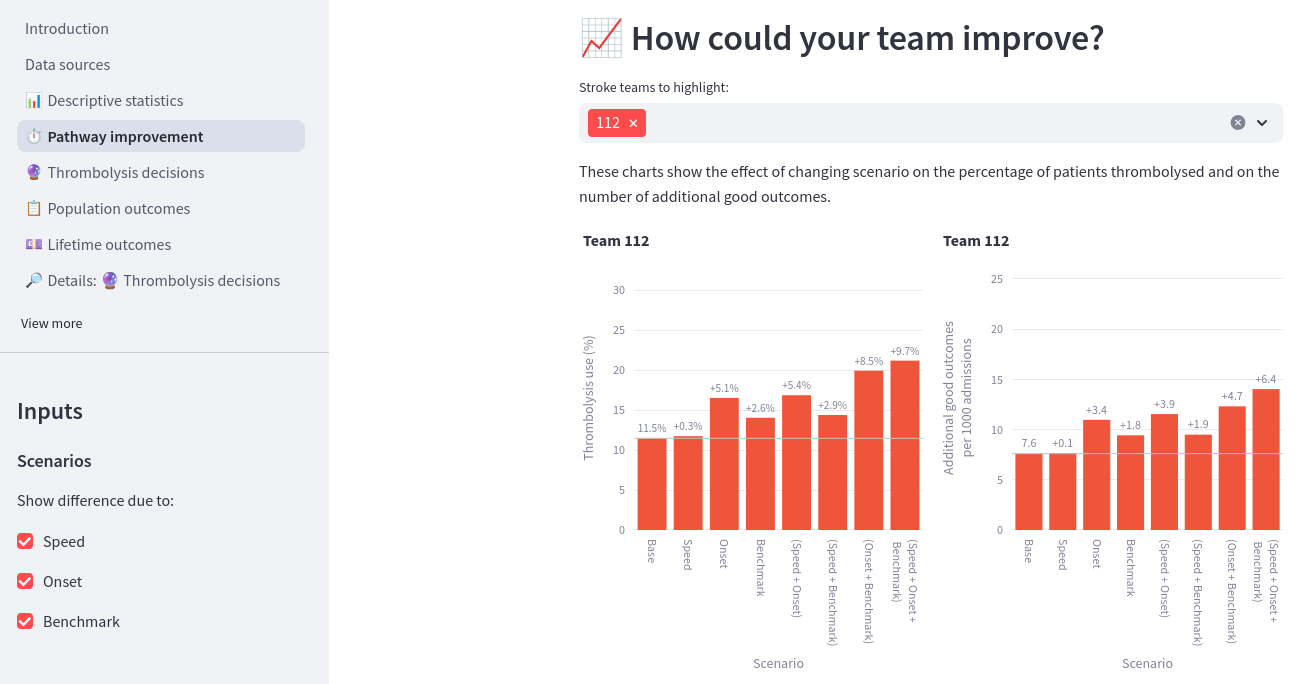
\includegraphics[width=0.75\linewidth]{images/web_app.png}
    \caption{Screenshot from a page of our current web application on improving thrombolysis use.}
    \label{fig:web_app}
\end{figure}

An example of feedback on presentation of the modelling available in the web app is shown below:

\begin{minipage}[t]{0.9\textwidth}
\begin{quote}
\textit{`Dear Martin (James). I just wanted to drop you a Thank You email for visiting our Trust today [to present the stroke audit machine learning and modelling work] with your colleagues; your presentation was superb, so inspirational in terms of the difference we can make for the patients who are not currently receiving thrombolysis; a great illustration of how we compare in our decision making to the ‘premier’ hospitals.....I think this is amazing work with huge clinical benefit. If it helps, I’d be very happy to provide a letter of support on behalf of the Trust/ISDN'.}

\vspace{5mm}

Ailsa Brotherton, Executive Director of Improvement, Research and Innovation, Improvement Director, National Improvement Board
\end{quote}
\end{minipage}

\subsection{Thrombolysis in Acute Stroke Collaborative (TASC)}

The SAMueL team has been providing bespoke reports to the \textit{Thrombolysis in Acute Stroke Collaborative} (TASC). TASC is an NHS-England sponsored and funded project working with NHS Elect. TASC is taking 6 low thrombolysing stroke teams and is helping them improve thrombolysis use. A follow up project, focussing on 12-15 more teams has been agreed.

\subsection{Conference presentations}

Work described here has been presented at the following conferences (presentations may be downloaded from the links provided):

Pearn, K., Allen, M., Laws, A., Everson, R. \& James, M. (2023). What would other emergency stroke teams do? Using explainable machine learning to understand variation in thrombolysis practice. European Stroke Organisation Conference. Zenodo. https://doi.org/10.5281/zenodo.7878306

Pearn, K., Allen, M., Laws, A., Everson, R. \& James, M. (2023). WHAT WOULD OTHER EMERGENCY STROKE TEAMS DO? Using explainable machine learning to understand variation in thrombolysis (clot-busting) practice. AI UK 2023 (Turing Institute), London, UK. Zenodo. https://doi.org/10.5281/zenodo.7759059

Pearn, K., Allen, M., Laws, A., \& James, M. (2024). VARIATION IN THROMBOLYSIS USE AND THE POTENTIAL EFFECT ON OUTCOMES IN ENGLAND AND WALES: AN OBSERVATIONAL MACHINE LEARNING STUDY. European Stroke Organisation Conference (ESOC). Zenodo. https://doi.org/10.5281/zenodo.11191491

Laws, A., Allen, M., Pearn, K., \& James, M. (2024). MODELLING DISABILITY-LEVEL AND UTILITY OUTCOMES DEPENDING ON TIME TO THROMBOLYSIS AND MECHANICAL THROMBECTOMY. European Stroke Organisation Conference (ESOC). Zenodo. https://doi.org/10.5281/zenodo.11191633

\section{Implications for decision makers}

\section{Research recommendations}

Recommendations for further research include:

\begin{itemize}

    \item How does variation in thrombolysis use (and resulting variation in outcomes) differ by population demographics?

    \item How does variation in thrombolysis use affect inpatient lengths of stay, and NHS bed use?

    \item How does use, benefit from, and bed use after, thrombectomy vary between admitting stroke team?

    \item Can causal inference methods (such as Directed Acyclic Graphs, propensity score adjustment, and target trial emulation) confirm the conclusions made in this project?

    \item How do we maximise uptake and impact of this work?
    
\end{itemize}


\section{Conclusions}

Using observational data and machine learning, thrombolysis was found to have at least as much benefit as predicted by the clinical trial meta-analysis. Variation in decision-making concerning thrombolysis is leading to significant between-hospital variation in thrombolysis use, and is leading to variation in outcomes. Stroke teams with higher thrombolysis use are predicted to be generating better patient outcomes. Clinicians were hopeful the SAMueL technology could address variance in thrombolysis practice. It was seen as particularly suitable for junior clinicians, non-stroke specialists and at district general hospitals and offered value for training, reviewing clinical cases, and quality improvement.

\section{Acknowledgements}

We would like to thank our Patient and Carer Involvement team led by Leon Farmer (David Burgess, Simon Douglas, Ian Hancock, Nicola Hancock, John Williams), and our expert advisory group (Ajay Bhalla, Gary Ford, Martin Utley).

\section{Declaration of conflicting interests}

The authors declare no potential conflicts of interest with respect to the research, authorship, and/or publication of this article. 

\section{Funding}

The authors disclose receipt of the following financial support for the research, authorship, and/or publication of this article: This research was funded by the National Institute for Health Research Applied Research Collaboration South West Peninsula and by the National Institute for Health Research Health and Social Care Delivery Research (HSDR) Programme [NIHR134326]. The views expressed in this publication are those of the authors and not necessarily those of the National Institute for Health Research or the Department of Health and Social Care. 